\chapter{Analiza wymagań}
Projektowany system powinien umożliwiać tworzenie ogłoszeń naborów do projektów, jak również dawać możliwość zarządzania samymi projektami. Aby zidentyfikować pełen zakres jego funkcji przeprowadzono przegląd istniejących rozwiązań powiązanych z poruszanym tematem. Pozwoliło to lepiej określić wymagania funkcjonalne i niefunkcjonalne dla tego systemu.

\section{Przegląd istniejących rozwiązań}
Na rynku znajduje się wiele platform, które w pewnym stopniu adresują ten problem, ale żadna z nich nie sprawia że użytkownicy znajdują się w pełnym środowisku do tworzenia projektów.
Osoby poszukujące innych osób do współpracy nad projektem musi korzystać z kilku niezależnych od siebie platform, co powoduje w dalszej perspektywie niepotrzebne kroki, utrudniające efektywne prowadzenie projektu.

\subsection{Github.com}
% TO DO: proszę korzystać ze spell-checkera (pojawia się za dużo literówek, które da się automatycznie poprawić)

Platforma założona przez Chrisa Wanstratha, P. J. Hyetta i Toma Prestona-Wernera w 2008 roku, która umożliwia hostowanie repozytoriów Git \cite{GitHub}. Użytkownicy mogą tworzyć własne repozytoria, przeglądać repozytoria innych użytkowników,
a także współpracować nad projektami poprzez zgłaszanie problemów (ang.~\emph{issues}), proponowanie zmian (ang.~\emph{pull requests}) oraz komentowanie kodu źródłowego.
W 2018 roku Github został wykupiony przez Microsoft, który wprowadził wiele zmian, m.in.\ brak limitu prywatnych repozytoriów dla użytkowników i wprowadzenie płatnych planów dla firm. W 2020 roku Github wprowadził funkcjonalność \emph{Github Actions}, która umożliwia automatyzację procesów związanych z tworzeniem oprogramowania, takich jak testowanie, budowanie i wdrażanie aplikacji.
Platforma ta umożliwia bardzo efektywną współpracę nad projektami, jednak nie oferuje ona możliwości tworzenia zgłoszeń zapotrzebowania na dane osoby w sposób ustrukturyzowany. Dużo projektów open-source
robi to w sposób nieformalny, często przez odpowiednią sekcję w pliku \texttt{README.md}. W kontekście problemu poruszanego w niniejszej pracy, to rozwiązanie jest niewystarczające, jednak ono jest adresuje najwięcej zdefiniowanych wymagań.

% TO DO: nazwy plików, kod źródłowy, elementy modeli itp. proszę pisać czcionką maszynową \texttt{}
%        wyróżnienia w języku angielskim proszę pisać korzystając z \emph{}
% Zostawiam komentarz żeby pamiętać na przyszłość - Filip

\subsection{JustJoin.It}
\label{sec:justjoin-it}
Portal z ogłoszeniami o pracę typowo w sferze IT \cite{JustJoinIt}. Oferuje efektywne filtry do ofert pracy i możliwość aplikacji do danej oferty z poziomu strony internetowej.
Firmy mogą w bardzo efektywny sposób publikować ogłoszenia z danymi ofertami pracy, gdzie samo ogłoszenie można sparametryzować do odpowiednich kryteriów wyszukiwania przez zainteresowanych.
Do takich parametrów należą m.in.: stack technologiczny, lokalizacja, tryb pracy typ umowy itp. Dla tego typu użytkowników jest to bardzo wygodne rozwiązanie ponieważ nie muszą poświęcać swoich środków marketingowych w celu
pozyskiwania nowych pracowników. Z kolei dla osoby poszukującej pracy, portal ten także jest wygodnym rozwiązaniem, ze względu na to że może on w prosty sposób wyszukać interesujące go ogłoszenie
za pomocą wcześniej wspomnianych filtrów. W kontekście problemu poruszanego w niniejszej pracy, rozwiązanie to nie jest w pełni kompleksowe.
Brakuje na nim narzędzi do zarządzania projektem i do hostowania kodu. Strona ta skupia się tylko na jednym podproblemie należącym do rozwiązywanego problemu.
Istotnym brakiem tej platformy, również jest grupa docelowa, a mianowicie nie są nią studenci poszukujący innych studentów do wspólnej nauki.
Główną grupą docelową w tym przypadku są osoby poszukujące pracy w branży, a także profesjonalne firmy poszukujące pracowników już z pewnym doświadczeniem.
Nie ma tam miejsca na typowo studenckie inicjatywy. 

\subsection{Jira}
Jira jest platformą firmy Atlassian przeznaczoną do zarządzania zadaniami i śledzenia postępu prac w projektach \cite{Jira}. Umożliwia organizowanie pracy w backlogu, planowanie sprintów oraz monitorowanie zgłoszeń.
W porównaniu z projektowanym systemem skupia się jednak na zarządzaniu realizacją projektu, a nie na wyszukiwaniu osób do zespołu i publikowaniu ogłoszeń rekrutacyjnych.

\subsection{Azure DevOps}
Zintegrowana platforma do zarządzania projektami i tworzenia oprogramowania, stworzona przez Microsoft. Oferuje ona narzędzia takie same jak Github, jednak poprzez grupę docelową (firmy) ma ona dużo bardziej rozwinięte narzędzia inne niż do hostowania kodu.
W porównaniu do Githuba, Azure devops ma dużo bardziej rozbudowane narzędzia do zarządzania zadaniami i odpowiedzalnością w projekcie. Poprzez prosty podział na zadania, platforma ta bardzo ułatwiła pracę w metodyce zwinnej (ang. \textit{Agile}). Rozwiązanie to niestety
jest płatne od ponad 5 użytkowników, co w kontekście projektów studencki stanowi pewne ograniczenie przy większej skali projektu. Dodatkowo studenci nie są grupą docelową takiego rozwiązania i mogą mieć problemy żeby w nim się odnaleźć.
Podobnie jak w przypadku Githuba, Azure DevOps nie oferuje możliwości tworzenia naborów osoby do projektu. W kontekście problemu poruszanego w niniejszej pracy, to rozwiązanie jest niewystarczające, jednak ono również adresuje dużo zdefiniowanych wymagań.

% TO DO: warto przegląd podsumować. można byłoby zrobić tabelę zbierającą cechy wszystkich rozwiązań (taką features table).
% TO DO: powinny pojawić się jakieś cytowania czy też adresy do stron omawianych systemów (by czytelnik mógł znaleźć szczegóły)
% DONE
\subsection{Podsumowanie przeglądu istniejących rozwiązań}
\label{sec:podsumowanie-przegladu}
Zestawienie cech omówionych platform przedstawiono w tabeli \ref{tab:porownanie-rozwiazan}.

\begin{table}[htb]
    \centering
    \caption{Porównanie funkcjonalności istniejących rozwiązań}
    \label{tab:porownanie-rozwiazan}
    \small
    \begin{tabularx}{\linewidth}{@{}X c c c c @{}}
        \toprule
        Funkcjonalność & GitHub & JustJoin.It & Jira & Azure DevOps \\
        \midrule
        Hosting repozytoriów \emph{Git}            & tak       & nie & nie       & tak       \\ \hline
        Tworzenie i śledzenie zadań               & tak       & nie & tak       & tak       \\ \hline
        Planowanie sprintów                        & częściowo & nie & tak       & tak       \\ \hline
        Role i uprawnienia w projekcie             & częściowo & nie & tak       & tak       \\ \hline
        Nabór osób do projektu                      & nie       & tak & nie       & nie       \\ \hline
        Aplikowanie na ogłoszenia                  & nie       & tak & nie       & nie       \\ \hline
        Filtrowanie ogłoszeń wg kryteriów          & nie       & tak & nie       & nie       \\ \hline
        Studenci jako grupa docelowa               & częściowo & nie & nie       & nie       \\ \hline
        Bezpłatność dla większych zespołów         & tak       & ---  & częściowo & nie      \\
        \bottomrule
    \end{tabularx}
\end{table}

Z przeprowadzonego przeglądu wynika, że żadna z omówionych platform nie łączy wszystkich funkcjonalności potrzebnych do rozwiązania problemu poruszanego w niniejszej pracy.
Platformy \emph{GitHub} i \emph{Azure DevOps} zapewniają hosting kodu i narzędzia do zarządzania zadaniami, przy czym \emph{Azure DevOps} oferuje bardziej rozbudowane wsparcie metodyki zwinnej, ale jest płatny powyżej 5 użytkowników.
\emph{Jira} skupia się wyłącznie na zarządzaniu realizacją projektu i nie umożliwia przechowywania kodu źródłowego.
Żadne z tych trzech narzędzi nie pozwala jednak publikować ogłoszeń o zapotrzebowaniu na osoby w projekcie.
Funkcjonalność tę oferuje portal \emph{JustJoin.It}, który z kolei nie posiada narzędzi do pracy nad projektem i jest skierowany do profesjonalnego rynku pracy, a nie do studentów.
W efekcie osoba chcąca zebrać zespół i prowadzić z nim projekt musi korzystać z co najmniej dwóch niezależnych platform.
Projektowany system ma wypełnić tę lukę, łącząc w jednym miejscu hosting repozytoriów, zarządzanie projektem oraz publikowanie ogłoszeń naborów i obsługę aplikacji.


\section{Założenia projektowe}

Projekt systemu zakłada że użytkownicy będą mogli tworzyć projekty, czyli podstawowe jednostki w systemie, na których będą opierali swoją pracę.
Pracując w danym projekcie, użytkownik będzie mógł tworzyć repozytoria, czyli miejsca w których będzie przechowywał kod źródłowy podlegający konkretnemu projektowi.
Oprócz kodu źródłowego użytkownik będzie mógł zarządzać projektem w metodyce zwinnej, czyli tworzyć sprinty i zadania, co pozwoli mu na efektywne zarządzanie pracą zespołu nad projektem.
W momencie kiedy zespół zauważy że brakuje im osoby o konkretnych umiejętnościach, będzie mógł stworzyć ogłoszenie o zapotrzebowaniu takiej osoby. Potem,
pod ogłoszeniem będą mogli sprawdzić kto aplikował na daną ofertę i w prosty sposób odsiać osoby które nie spełniają wymagań. W momencie kiedy zespół znajdzie pożądaną osobę,
w prosty sposób będzie mógł ją dodać do projektu i przydzielić jej odpowiednią, zdefiniowaną wcześniej rolę.


\subsection{Wymagania funkcjonalne i niefunkcjonalne}
W celu rozwiązania omawianego problemu, tworzony system musi oferować połączenie kilku niezależnych od siebie funkcjonalności, takich jak hosting repozytoriów,
zgłaszania zapotrzebowania na osoby w projekcie, wyszukiwania takich ofert i podstawowego zarządzania projektem w postaci rozpisywania zadań i przydzielania odpowiedzialności za nie.
W tym celu przeprowadzono analizę wymagań funkcjonalnych i niefunkcjonalnych. Po analizie założeń projektowych zdefiniowano wymagania funkcjonalne przedstawione w tabeli~\ref{tab:wymagania-funkcjonalne}.
Tabela ma postać tabeli wymagań SysML: każde wymaganie ma identyfikator (\texttt{id}), nazwę, treść (\texttt{text}) oraz wskazanie wymagania nadrzędnego, w którym jest zawarte.
Identyfikatory odpowiadają blokom na diagramie z rysunku \ref{fig:sysml_wymag}. Wymagania niefunkcjonalne zestawiono w tabeli \ref{tab:wymagania-niefunkcjonalne}.
% TO DO: $...$ - to otoczenie matematyczne, proszę go nie stosować jeśli chce Pan wyróżnić jakąś nazwę, bo zamiast czcionki maszynowej czy kursywy pojawi się czcionka matematyczna (używana przy pisaniu wzorów)
% Podobnie jak wyżej - zostawiam żeby pamiętać i mieć to pod ręką - Filip
\begin{table}[htb]
    \centering
    \caption{Wymagania funkcjonalne systemu}
    \label{tab:wymagania-funkcjonalne}
    \small
    \begin{tabularx}{\linewidth}{@{}l >{\raggedright\arraybackslash}p{3.5cm} >{\raggedright\arraybackslash}X c@{}}
        \toprule
        Id & Nazwa & Treść (\texttt{text}) & Nadrzędne \\
        \midrule
        1     & System & System umożliwia publikowanie ogłoszeń naborów do projektów oraz zarządzanie projektami programistycznymi & --- \\
        \midrule
        1.1   & Dostęp do systemu       & System kontroluje dostęp użytkowników do platformy & 1 \\
        1.1.1 & Konto użytkownika       & System wymaga założenia konta & 1.1 \\
        1.1.2 & Przeglądanie projektów  & Biznes przegląda projekty & 1.1 \\
        \midrule
        1.2   & Hosting repozytoriów    & System hostuje repozytoria systemu kontroli wersji \emph{Git} & 1 \\
        1.2.1 & Operacje \emph{Git}     & System obsługuje komendy \texttt{push}, \texttt{pull} i \texttt{clone} systemu kontroli wersji \emph{Git} & 1.2 \\
        1.2.2 & Import z \emph{GitHub}  & System importuje repozytoria z platformy \emph{GitHub} & 1.2 \\
        \midrule
        1.3   & Kontrola dostępu \emph{RBAC} & System implementuje \emph{RBAC} dla każdego projektu & 1 \\
        1.3.1 & Dynamiczne role         & System definiuje dynamicznie role w projekcie & 1.3 \\
        1.3.2 & Nadawanie ról           & Członek projektu z uprawnieniami nadaje role w projekcie & 1.3 \\
        1.3.3 & Zarządzanie członkami   & Członek projektu z uprawnieniami dodaje i usuwa osoby w projekcie & 1.3 \\
        1.3.4 & Zaproszenia e-mail      & System wysyła zaproszenia do projektu na maila & 1.3 \\
        \midrule
        1.4   & Ogłoszenia naborów      & Członek projektu publikuje oferty pracy w projekcie & 1 \\
        1.4.1 & Aplikowanie na ofertę   & Użytkownik może aplikować na daną ofertę & 1.4 \\
        1.4.2 & Przegląd aplikacji      & Członek projektu widzi aplikacje na daną ofertę & 1.4 \\
        \midrule
        1.5   & Planowanie pracy        & System umożliwia planowanie pracy zespołu w projekcie & 1 \\
        1.5.1 & Sprinty                 & Członek projektu tworzy sprinty & 1.5 \\
        1.5.2 & Zadania                 & Członek projektu tworzy zadania & 1.5 \\
        \bottomrule
    \end{tabularx}
\end{table}

\begin{table}[htb]
    \centering
    \caption{Wymagania niefunkcjonalne systemu}
    \label{tab:wymagania-niefunkcjonalne}
    \small
    \begin{tabularx}{\linewidth}{@{}l >{\raggedright\arraybackslash}p{3.5cm} >{\raggedright\arraybackslash}X@{}}
        \toprule
        Id & Nazwa & Treść (\texttt{text}) \\
        \midrule
        NF1 & Przechowywanie repozytoriów & System przechowuje repozytoria na serwerze \\
        NF2 & Magazyn plików              & System przechowuje pliki dla aplikacji w magazynie chmurowym \\
        NF3 & Integracja z \emph{GitHub}  & System zapewnia integrację z platformą \emph{GitHub} \\
        NF4 & Wydajność                   & System zapewnia przepustowość dla wielu użytkowników \\
        NF5 & Bezpieczeństwo              & System zapewnia bezpieczeństwo danych użytkowników \\
        NF6 & Metodyka zwinna             & System umożliwia zarządzanie projektem metodyką zwinną \\
        \bottomrule
    \end{tabularx}
\end{table}

\subsection{Diagram SysML wymagań funkcjonalnych}
W celu lepszej wizualizacji wymagań funkcjonalnych, na rysunku~\ref{fig:sysml_wymag} przedstawiono diagram SysML obrazujący powiązania między poszczególnymi modułami. 
\begin{figure}[htb]
    \centering
    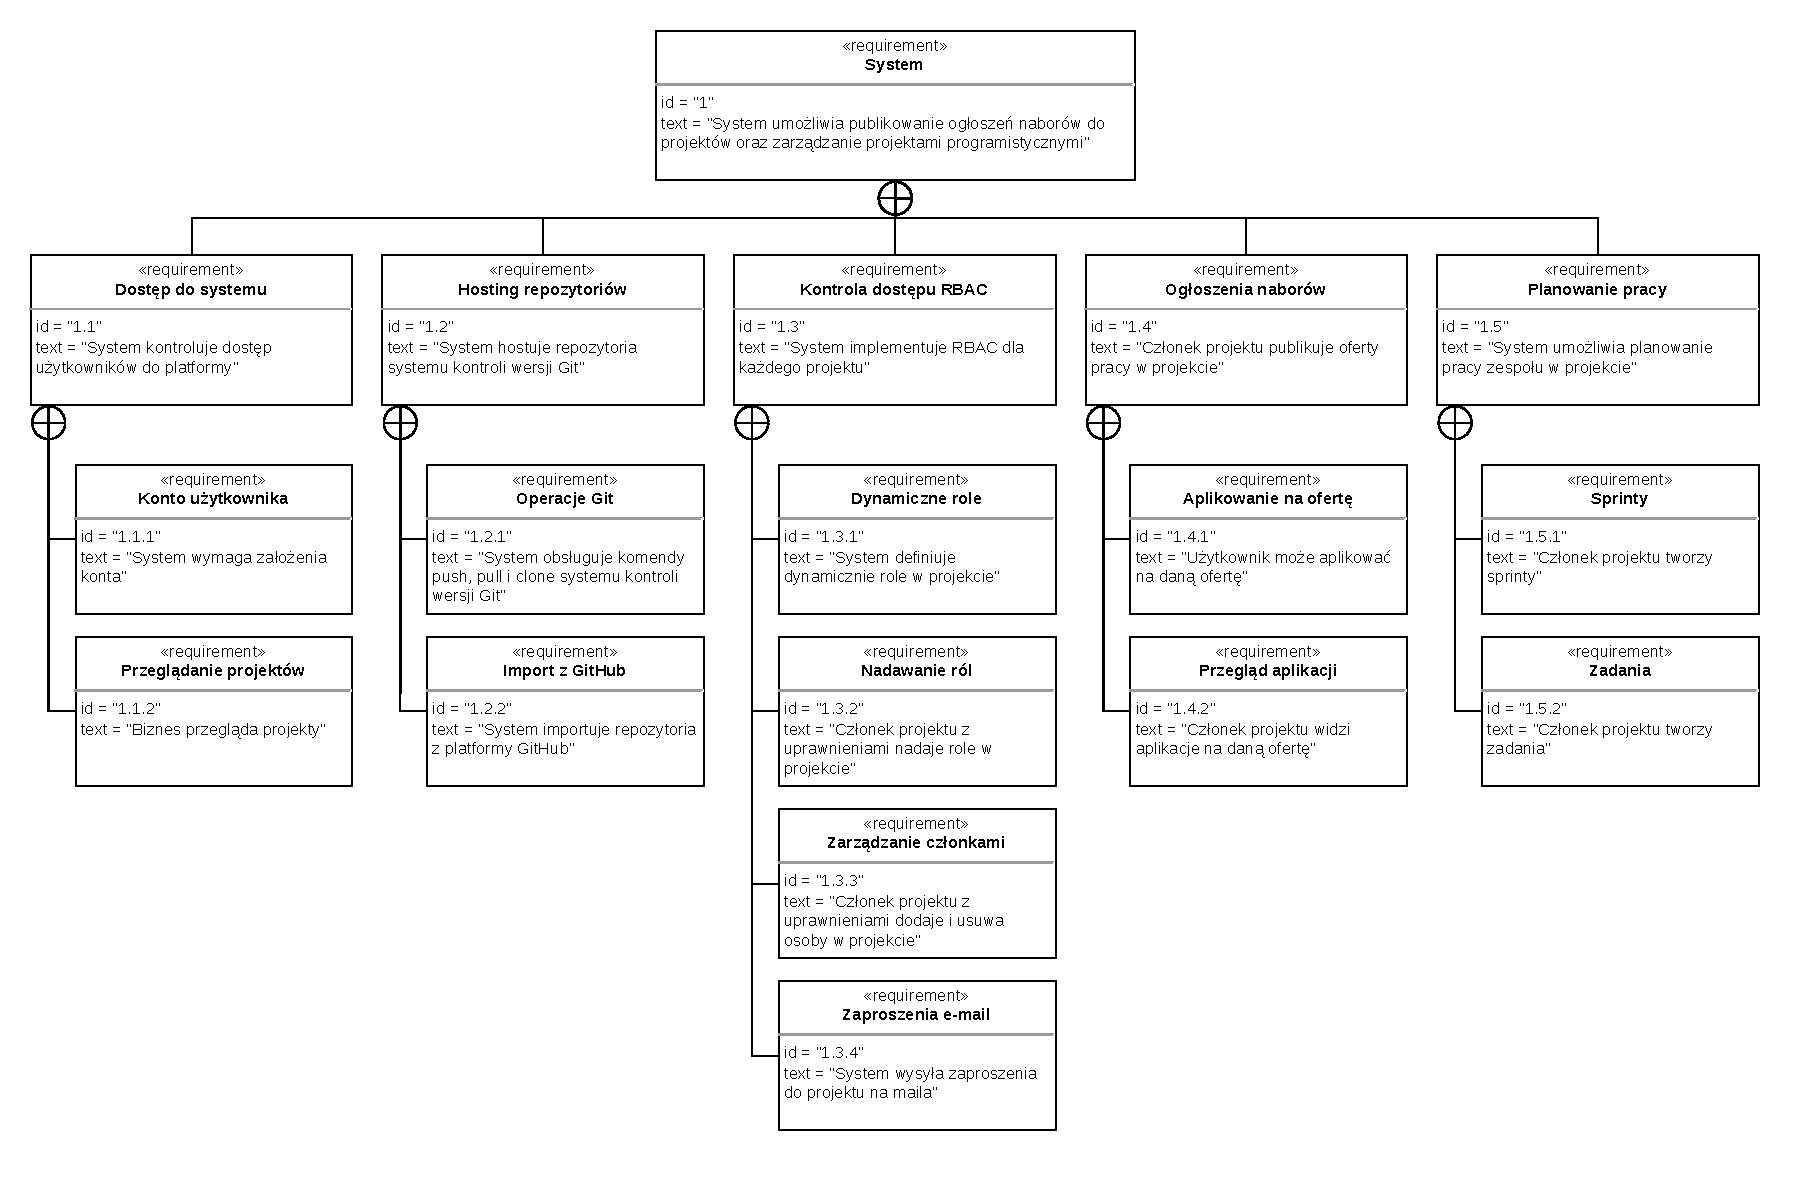
\includegraphics[scale=0.5]{rys02/sysML_wymagania.drawio-1.pdf}
    \caption{Diagram SysML wymagań funkcjonalnych}
    \label{fig:sysml_wymag}
\end{figure}
% TO DO: w specyfikacji "SysML requirements diagram" atrybuty id oraz text są OBOWIĄZKOWE.
%        proszę uzupełnić te atrybuty na diagramie
%        symbol klasy nie jest wymagany (C)
%        nie wiem, w czym zrobiony został diagram, zamiast grafiki rastrowej dobrze byłoby mieć grafikę wektorową pdf
%        SysML pozwala zapisać wymagania w tabeli. Przy dużej liczbie wymagań to lepsze niż diagram.
%        nawiasem mówiąc sam diagram da się lepiej narysować - obecny ma za dużo białej przestrzeni (bloczki można pozacieśniać, opisy mogą być wielolinijkowe itd.
%        https://re-magazine.ireb.org/articles/modeling-requirements-with-sysml
% DONE
\subsection{Przypadki użycia}
Po zdefiniowaniu wymagań, na ich podstawie powstały następujące przypadki użycia na rysunku~\ref{fig:przypadki}:
\subsubsection{Diagram przypadków użycia}
%TODO rozpisać przypadki użycia?

%TODO: Skalowanie i ustawienie obu obrazków
\begin{figure}[htb]
    \centering
    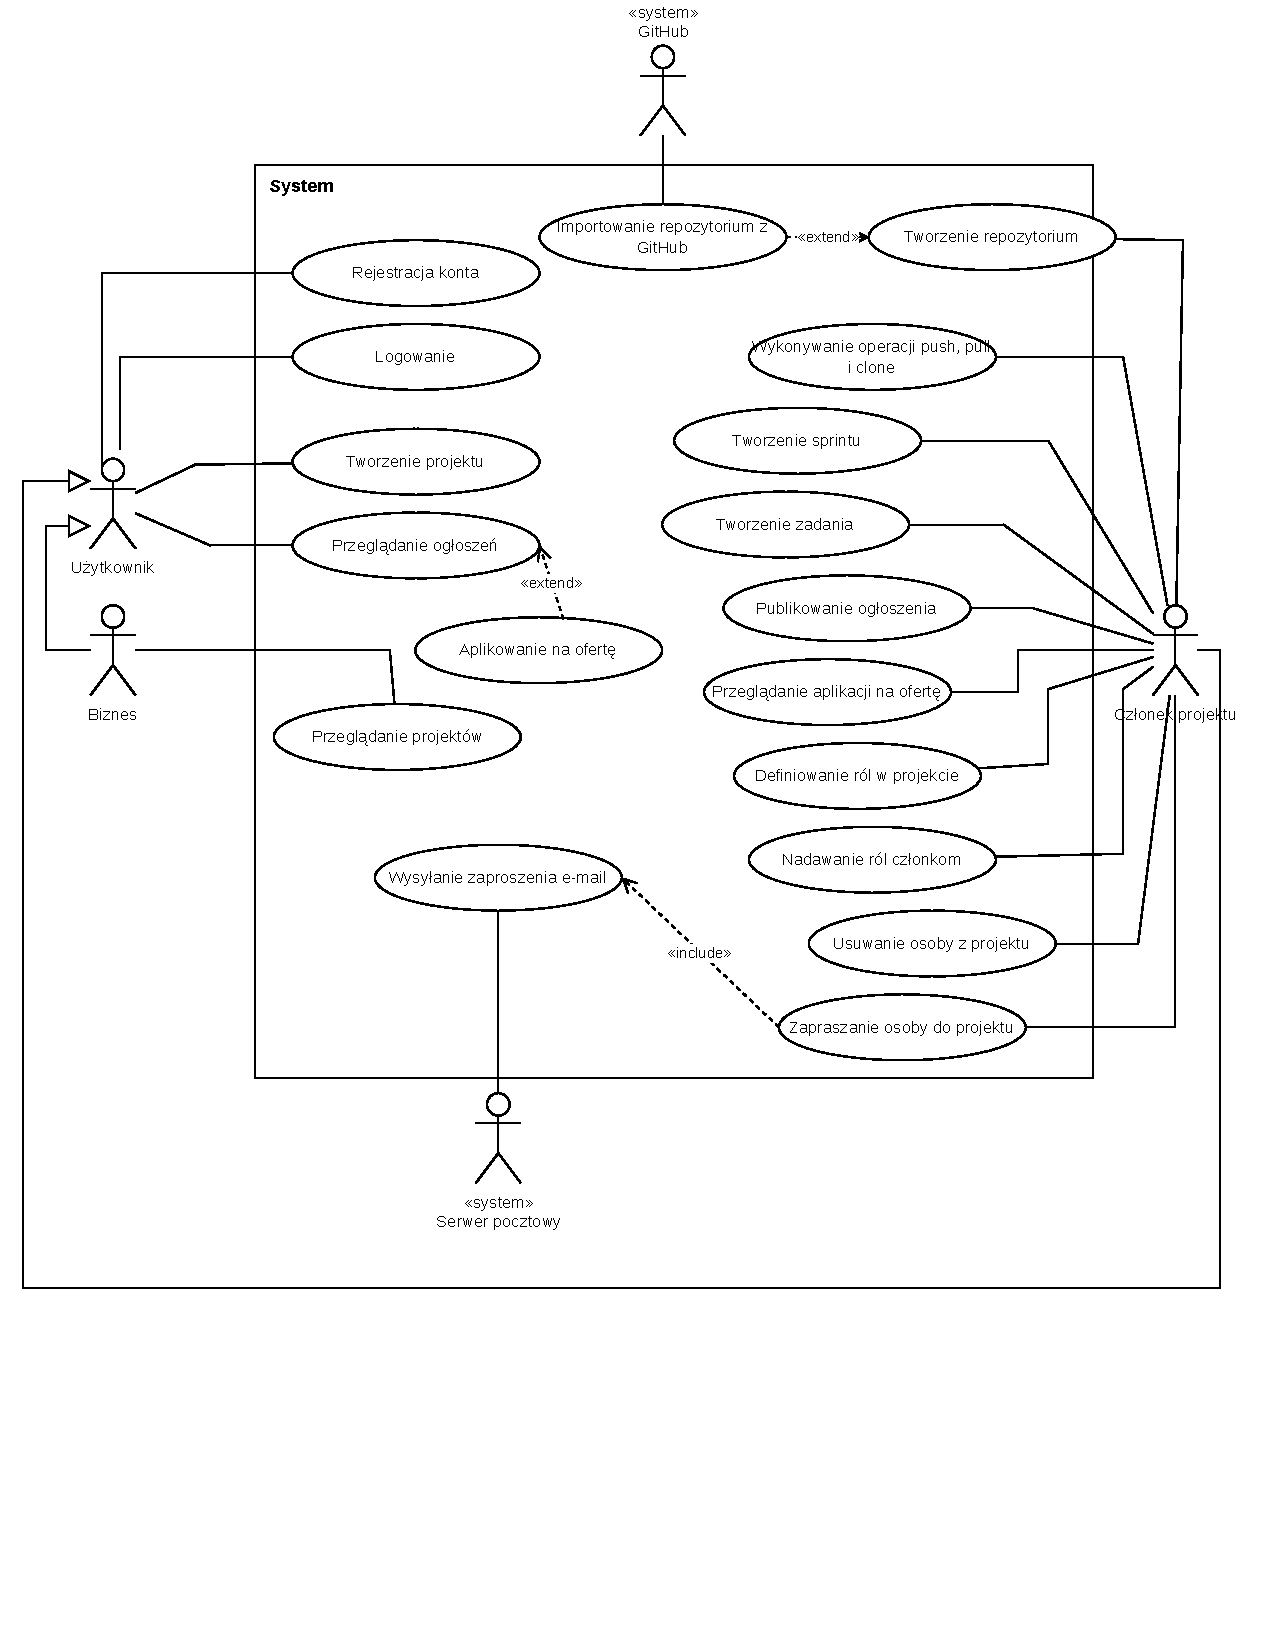
\includegraphics[scale=0.5]{rys02/przypadki.drawio.pdf}
    \caption{Diagram SysML wymagań funkcjonalnych}
    \label{fig:przypadki}
\end{figure}